\chapter{Применение} \label{chapt3}
\section{Распознавание символов}
В рамках разработки алгоритмов распознавания была спроектированна база данных для хранения информации об образцах и разработан комплекс программ для проверки практической применимости разработанных методов. 

База реализованна с использованием СУБД MSSQL. Проект БД приведен в приложении А.

Комплекс ПО состоит из трех программ:
\begin{enumerate}
\item Конвертор растровых изображений
\item Браузер для базы данных
\item Интерпретатор 
\end{enumerate}
Все три программы написанны на языке C++. В качестве GUI используется Borland VLC. Программы используют общую базу данных, доступ к которой осуществляется через ODBC, что позволяет использовать любую совместимую СУБД.

\subsection{Конвертор растровых изображений}
\noindent
Осуществляет преобразование растрового изображения в а.с. вида \ref{eq:model}. В программе присутствует простой графический редактор.

\begin{figure}[h]
	\centering
	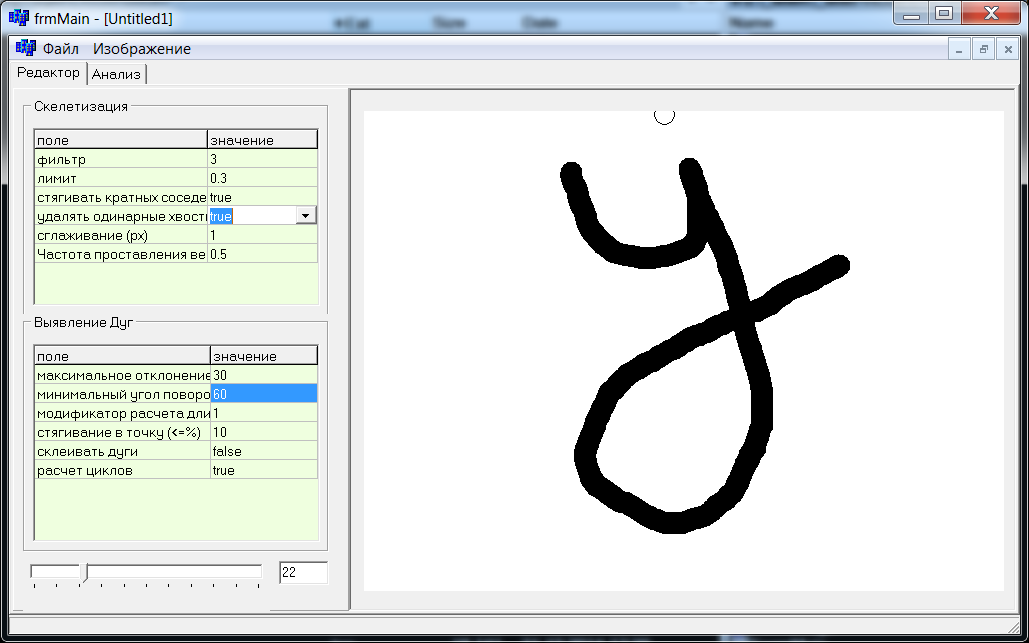
\includegraphics[scale=0.25]{images/an_convertor_2}
	\caption{Графический редактор}
	\label{em_img_program}
\end{figure}

\begin{figure}[h]
%	\centering
	\begin{subfigure}{.5\textwidth}
%		\centering
		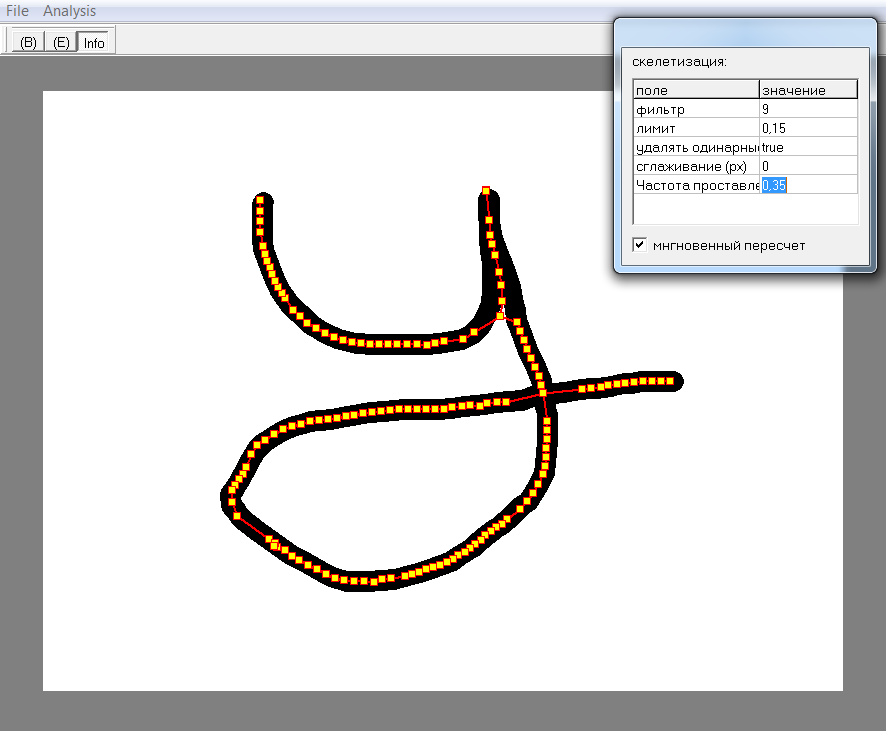
\includegraphics[width=\linewidth]{images/an_convertor_graph_2.png}
		\caption{шаг: 0.35 от ширины волны}
	\end{subfigure}
	\begin{subfigure}{.5\textwidth}
%		\centering
		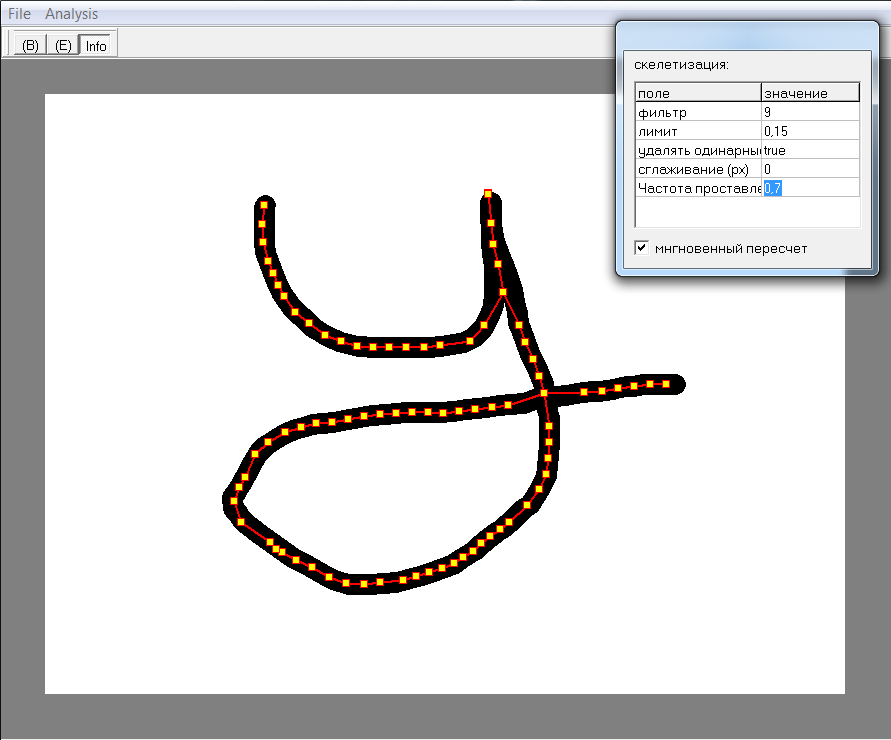
\includegraphics[width=\linewidth]{images/an_convertor_graph_1.png}
		\caption{шаг: 0.75 от ширины волны}
	\end{subfigure}
	\caption{Разный шаг аппроксимации графа}
\end{figure}

Нарисованное изображение можно преобразовать в систему дуг и связей дуг.

\begin{figure}[h]
%	\centering
	\begin{subfigure}{.45\textwidth}
		\centering
		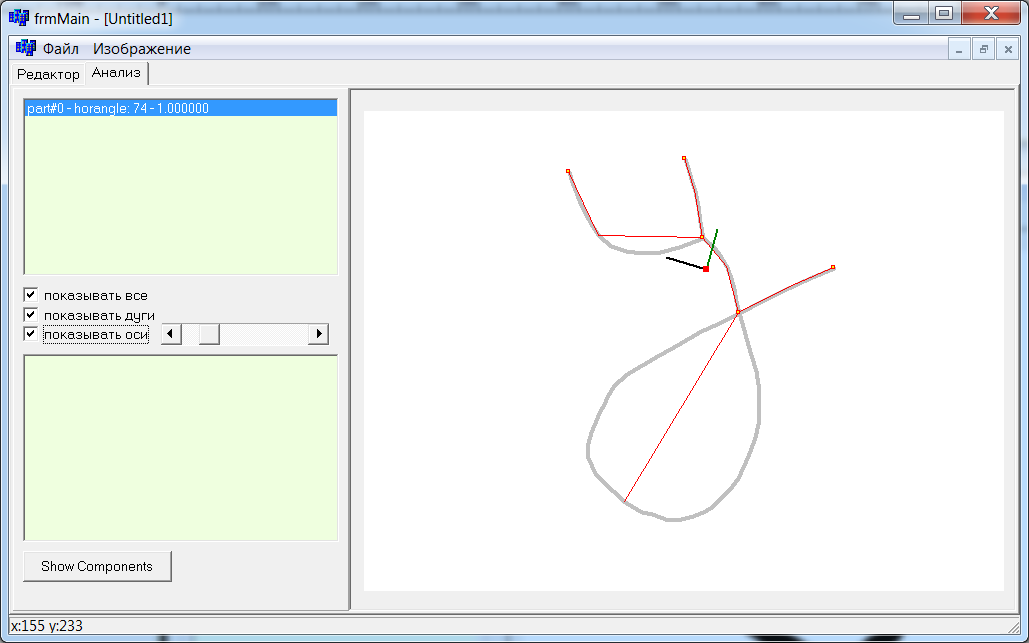
\includegraphics[width=.9\linewidth]{images/an_convertor_1.png}
		\caption{Преобразованное изображение, нарисованное поверх исходного}
	\end{subfigure}
	\begin{subfigure}{.45\textwidth}
		\centering
		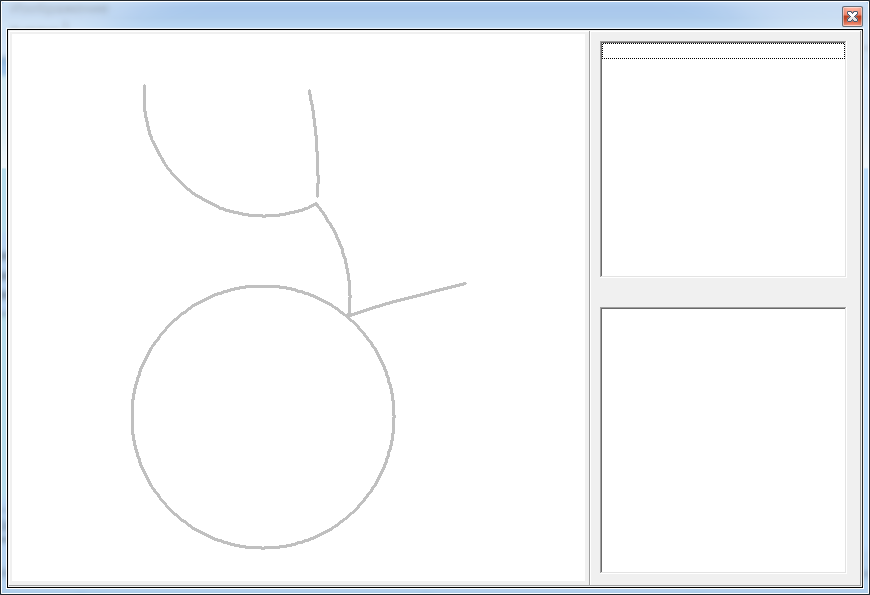
\includegraphics[width=.9\linewidth]{images/an_convertor_3.png}
		\caption{Преобразованное изображение, нарисованное по набору дуг и связей между ними}
	\end{subfigure}
	\caption{Преобразованное изображение}
\end{figure}

Также программа обладает системой простого обучения. Обучение осуществляется путем сопоставления соответствующих дуг. Как результат обучения в БД в качестве изображения отправляется система, где всякой дуге сопоставляется не конкретное значение сектора, а некий промежуток значений.

Преобразованное изображение можно сохранить в БД в качестве нового образца.

\begin{figure}[h]
	\centering
	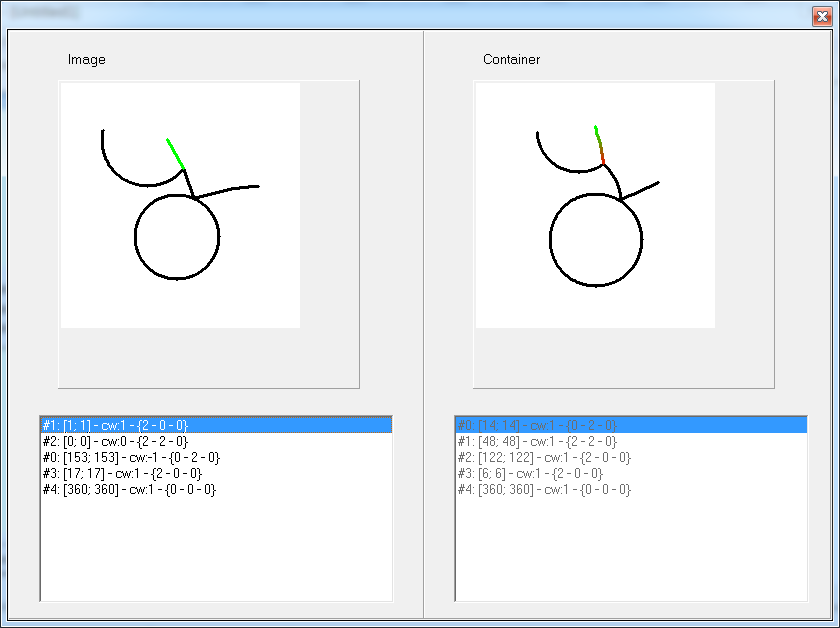
\includegraphics[scale=0.35]{images/an_convertor_4}
	\caption{Обучение системы}
\end{figure}

\subsection{Браузер для БД}
Используется для просмотра образцов хранящихся в БД. 
Наглядно отображает связи в изображении, и умеет пересчитывать их относительно выбранной дуги. Интерфейс программы можно посмотреть на рис. \ref{an:preview}.
\begin{figure}[h]
%	\centering
	\begin{subfigure}{.5\textwidth}
		\centering
		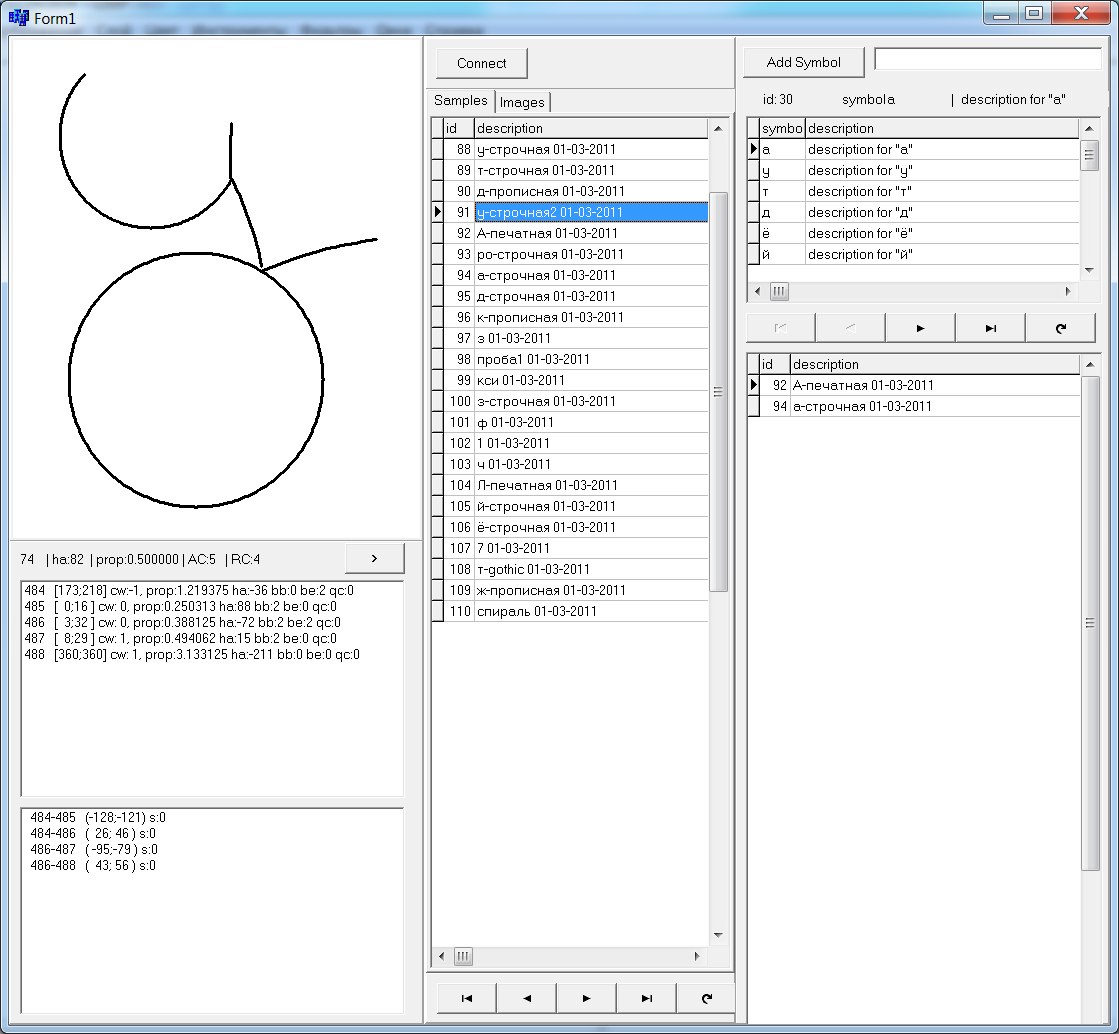
\includegraphics[width=.9\linewidth]{images/an_preview_1}
		\caption{Изображение построенное по набору дуг и связей между ними}
	\end{subfigure}
	\begin{subfigure}{.5\textwidth}
		\centering
		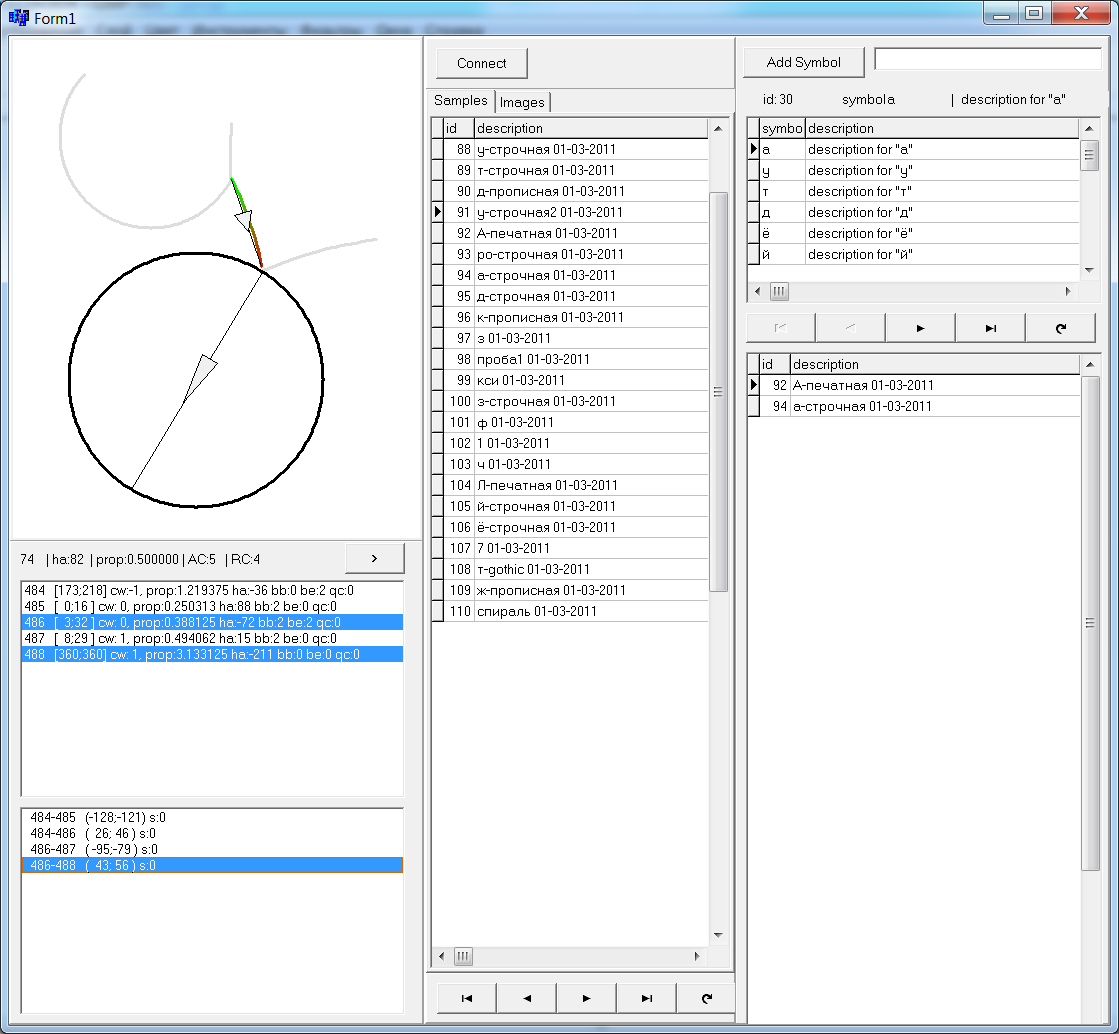
\includegraphics[width=.9\linewidth]{images/an_preview_2}
		\caption{Связь между дугой и круговой дугой (360 градусов)}
	\end{subfigure}
	\begin{subfigure}{1\textwidth}
			\centering
			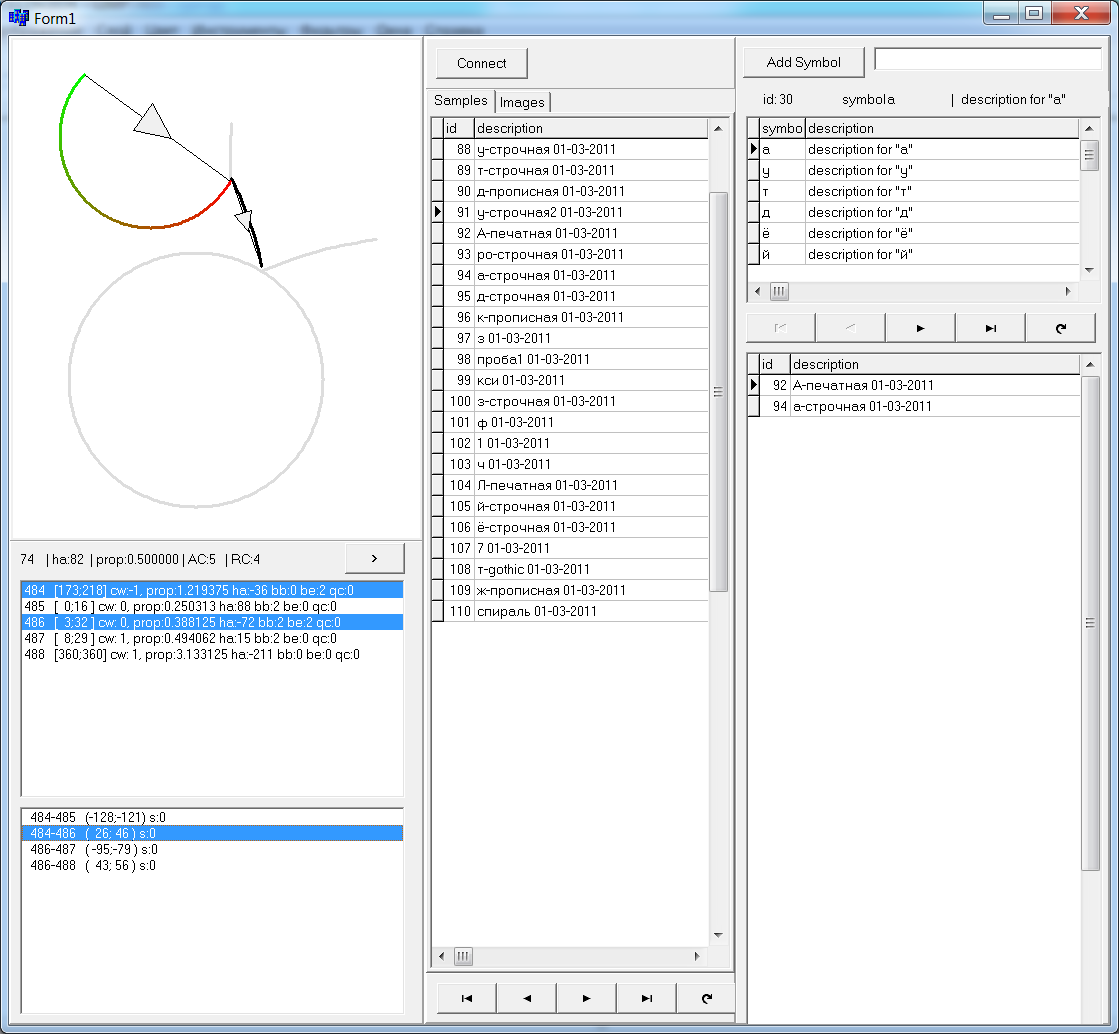
\includegraphics[width=.45\linewidth]{images/an_preview_3}
			\caption{Связь между двумя дугами}
	\end{subfigure}
	\caption{Преобразованное изображение}
	\label{an:preview}
\end{figure}


\subsection{Интерпретатор}
Предназначен для сопоставления анализируемого изображения с анализируемым образцом. В интерпретаторе реализованы алгоритмы, рассмотренные в параграфе 2.5.
Программа считывает данные из БД образцов в локальную БД и осуществляет сопоставление обработанного изображениями с образцами хранящимися в БД. Интерфейс изображение представлен на рис. \ref{an:analyze}.

\begin{figure}[h]
	\centering
	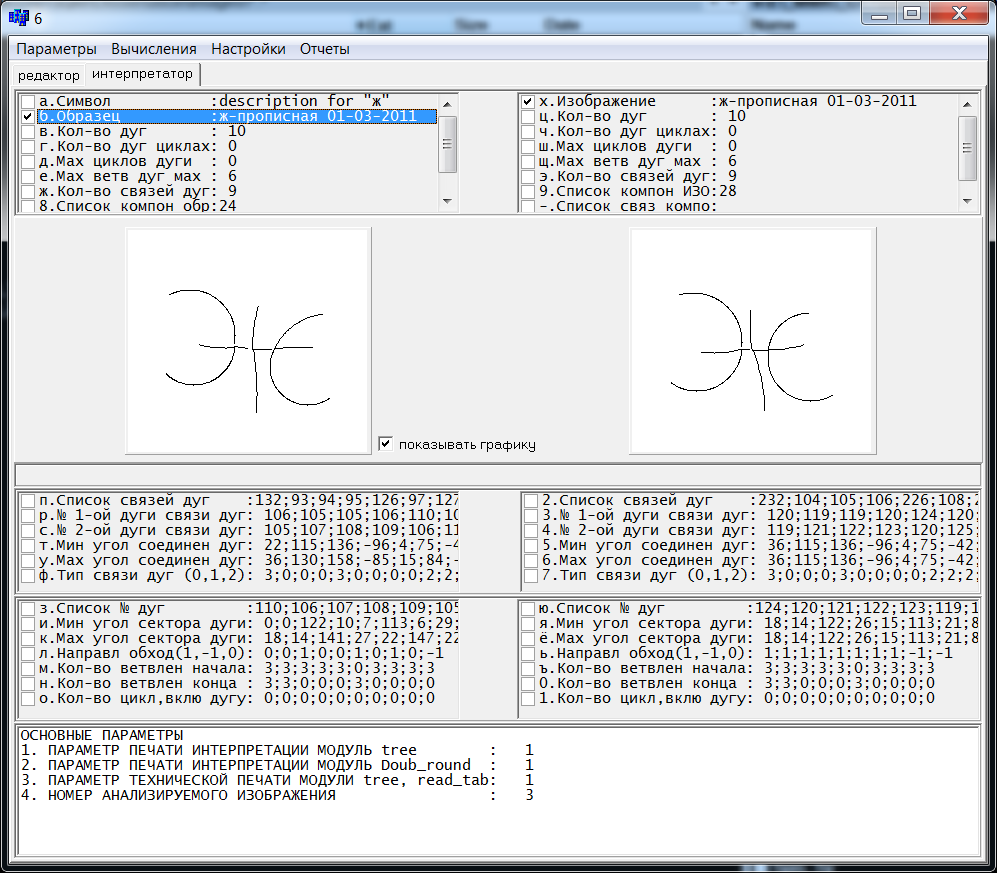
\includegraphics[scale=0.25]{images/an_convertor_analyze}
	\caption{Интерфейс интерпретатора}
	\label{an:analyze}
\end{figure}

\section{Оценка устойчивости битумных эмульсий}
\subsection{Введение}
В настоящее время трудно назвать область строительства, где бы не применялись эмульсии. Они используются в дорожном и в гражданском строительстве в качестве связующих с различными наполнителями, а также в качестве гидроизоляционных и лакокрасочных материалов. При любых технологиях использования эмульсий мы сталкиваются с одними и теми же проблемами, касающимися подбора состава, приготовления, определения физико-механических характеристик, стабильности, контроля распада эмульсий и получения продукции с необходимыми свойствами [1]. Далее мы будем рассматривать только прямые битумные и битумно-латексные эмульсии, которые являются наиболее крупнотоннажным продуктом: мировое использование составляет миллионы тонн в год

Традиционные методы оценки свойств битумных эмульсий включают: определение содержания вяжущего с эмульгатором, определение устойчивости эмульсии при перемешивании, определение остатка на сите, определение условной вязкости, определение устойчивости при хранении, определение адгезии эмульсий с поверхностью наполнителей, определение устойчивости при транспортировки и т.п. [2].  Наряду с традиционными методами изучения  качества эмульсии, во многих приложениях желательно знать более тонкие характеристики, например: функцию распределения по размерам. Эта характеристика является одним из важнейших параметров и позволяет предсказывать большинство свойств эмульсии. Обычноразмер частиц оценивают с помощью определения остатка на сите с заданным размером ячейки, но такой метод позволяет оценивать только верхний предел размеров частиц эмульсии. Полная картина распределения частиц по размеру может быть измерена с использованием таких технических приёмов как рассеяние света, микроскопия с анализом изображений, или же с помощью техники электроозонирования («техники Культера» - Coulter). Точный анализ размеров частиц битумной эмульсии может решить многие проблемы, которые в настоящее время являются актуальными в сфере производства битумных эмульсий:
\begin{enumerate}
\item Влияние эмульгатора и его концентрации на размер битумных частиц эмульсии.
\item Влияние модифицирующих битум добавок на качество получаемой эмульсии.
\item Корректировка технологической схемы производства эмульсии.
\item Влияние размера битумных частиц на основные физические свойства эмульсии.
\end{enumerate}

Оптическая микроскопия, как способ распределения частиц по размерам, является наиболее удобным и точным.Например, если в способе «рассеяние света» могут возникнуть проблемы с отражением света от черных поверхностей, какими являются частицы битума, то в способе микроскопии, при высоком контрасте черного цвета, напротив, можно отличить частицы от среды, в которой они находятся.

\begin{figure}[h]
	\centering
	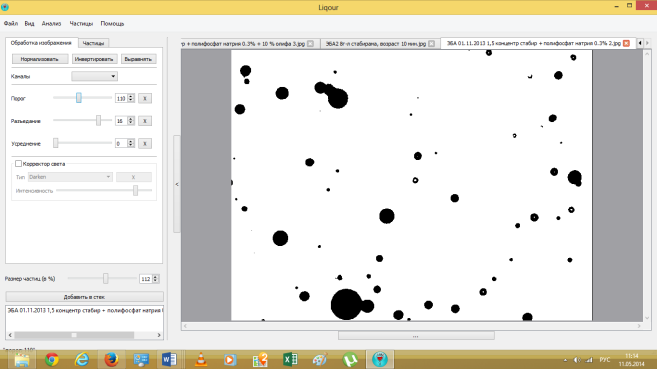
\includegraphics{images/em_00}
\end{figure}

Очевидно изображения такого вида являются одним из примеров растровых контурных изображений, с несколькими контурами. В отличие от задачи распознавания символов, здесь нет необходимости анализировать скелет изображения. Куда более важную роль играет внешний контур. Разбивая контур на дуги мы можем классифицировать частицы по уровню распада:
\begin{enumerate}
\item одиночные
\item слипшиеся
\item распавшиеся
\end{enumerate}
Большое количество распавшихся частиц является свидетельством того что смесь является неустойчивой, а следовательно некачественной.

\subsection{Анализ эмульсий}
В результате сотрудничества с кафедрой <<Автомобильных дорог>> НИ ИрГТУ была разработана программа для первичной оценки качества битумных эмульсий

\begin{figure}[h]
	\centering
	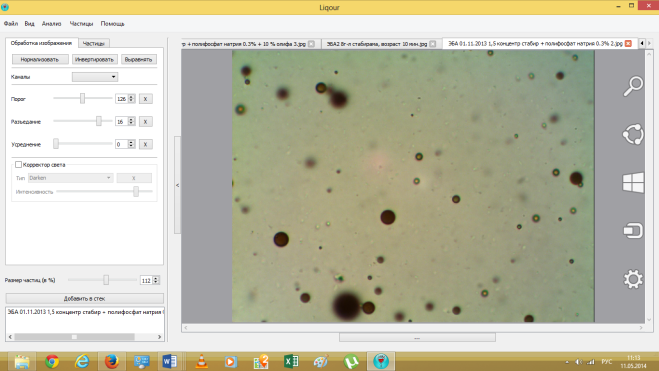
\includegraphics{images/em_03}
	\caption{Скриншоты программы «анализ изображений»}
	\label{em_img_program}
\end{figure}

\begin{figure}[h]
	\centering
	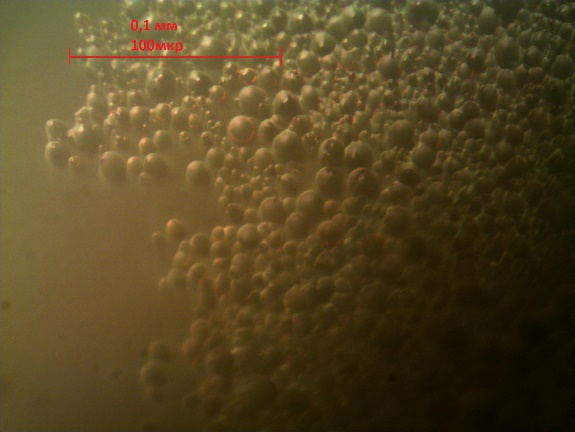
\includegraphics{images/em_01}
	\caption{Концентрированная битумная анионная эмульсия в отраженном свете}
	\label{em_img_bad}
\end{figure}

На снимке программы (рис. \ref{em_img_program}), видно, что в проходящем свете частицы легко отличить друг от друга, но для получения такого изображения необходимо создать некоторое пространство между ними, в противном случае изображение получатся как на рис. \ref{em_img_bad}. Поэтому перед микроскопическими исследованиями образцы эмульсии распределяют небольшим количеством (концентрация от 1:100 – 1:50) в специальном стабилизирующем растворе. Необходимость данной процедуры объясняется тем что, частицы битума могут слипаться под стеклышком и отсутствие сцепления между ними осуществляется за счет pH среды, в которой они находятся. Для анионных эмульсий это pH-щелочной, для катионных pH-кислотный.

Гибкость настроек программы позволяет редактировать изображение вручную, убирая «мнимые частицы», затемненные области и другие недочеты фотосъемки. После чего происходит автоматический подсчет частиц и построение графика функции распределения по размерам, рис. 5. 

Для данной программы не требуется специализированного оборудования. Достаточно оптического микроскопа с возможностью подключения цифровой камеры и компьютер с ОС (Windows, Linux, OS).

\subsection{Оценка качества анализа}

\begin{figure}[ht]
	\centering
	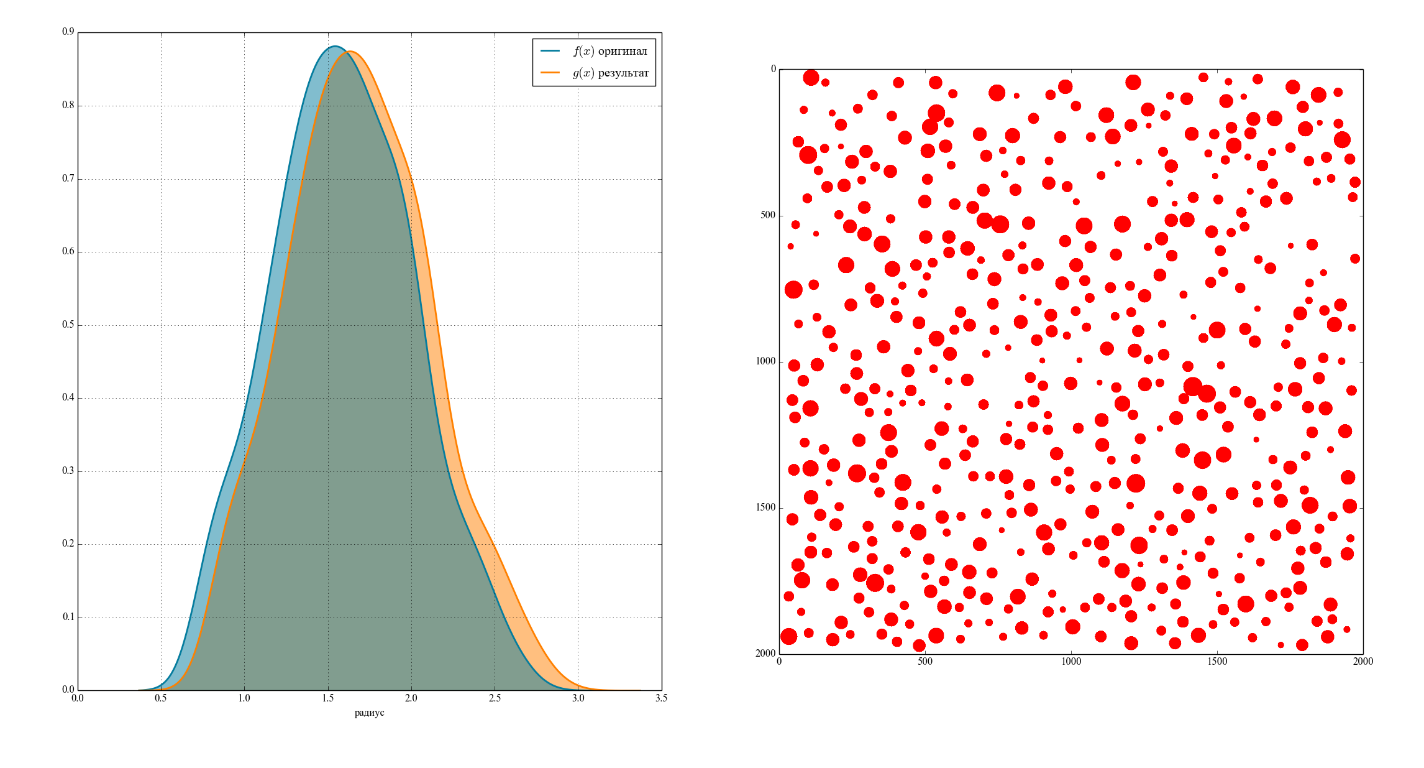
\includegraphics{images/em_07}
	\caption{Результат работы программы на искусствено сгенерированных данных}
	\label{em_artifical}
\end{figure}

На рисунке (рис. \ref{em_artifical}) приведены два графика: тот что сильнее смещен влево – соответствует исходным авто-сгенерированным данным, смещенный вправо соответствует распознанным данным. Формы графиков практически идентичны. Смещение, как правило, вызвано ошибками округления при распознавании объектов.

\begin{table}[ht]
  \centering
  \caption{Анализ распределения частиц на рис. \ref{em_artifical}}
  \renewcommand{\arraystretch}{1.5}% Spread rows out...
  \begin{tabular}{*5{>{\centering\bfseries}m{1in}}>{\centering\arraybackslash}m{0.6in}}
    \toprule
	График & \textbf{мин. размер частиц, мкм.} & \textbf{макс. размер частиц, мкм.} & \textbf{Среднее значение, мкм.} & \textbf{Ср.кв. отклонение, мкм.} & \textbf{Всего частиц} \\
	\midrule
	\midrule	
	Исходный & 0.87 & 2.87 & 1.69 & 0.42 & 500 \\
	Распознанный & 0.87 & 2.69 & 1.59 & 0.41 & 493 \\
	\bottomrule
  \end{tabular}
\end{table}

\begin{figure}[ht]
	\centering
	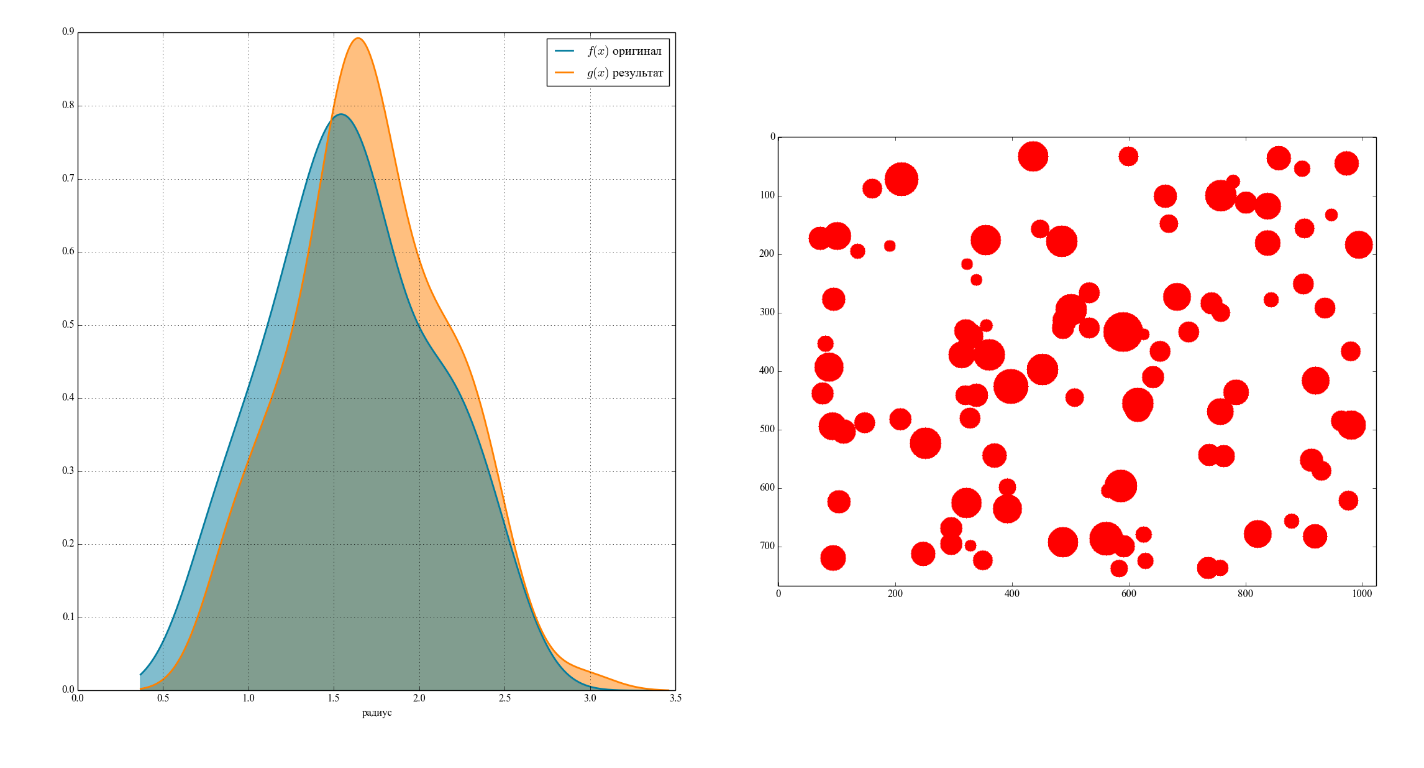
\includegraphics{images/em_04}
	\caption{Проверка работы программы при наличии слипшихся частиц}
	\label{em_merged}
\end{figure}


Вторым фактором (первый – ошибки округления) отрицательно влияющим на качество распознавания является наличие слипшихся частиц. На рис.\ref{em_merged} приведены два графика исходного (тот что более сплющен) и распознанного распределения частиц (тот что повыше). Сильное различие между графиками обусловлено тем что, при распознавании слипшиеся объекты не учитываются. 


\begin{table}[ht]
  \centering
  \caption{Распределение частиц на рис. \ref{em_merged}}
  \renewcommand{\arraystretch}{1.5}% Spread rows out...
  \begin{tabular}{*5{>{\centering\bfseries}m{1in}}>{\centering\arraybackslash}m{0.6in}}
    \toprule
	График & \textbf{мин. размер частиц, мкм.} & \textbf{макс. размер частиц, мкм.} & \textbf{Среднее значение, мкм.} & \textbf{Ср.кв. отклонение, мкм.} & \textbf{Всего частиц} \\
	\midrule
	\midrule
	Исходный & 0.87 & 2.98 & 1.71 & 0.44 & 100 \\
	Распознанный & 0.87 & 2.52 & 1.6 & 0.46 & 57 \\
	\bottomrule
  \end{tabular}
  \label{em_tbl_merged}
\end{table}

Из таблицы \ref{em_tbl_merged} видно, что, не смотря на то, что почти половина частиц не была распознана, характеристики распределения были определены достаточно точно к исходным, и погрешность составила около 4-5\%.

Получение высококачественной, долговечной битумной эмульсии зависит в основном от вязкости битума поступающего в диспергатор вместе с раствором ПАВ, а так же от скорости вращения и вида диспергирующих элементов. После выхода готовой эмульсии из диспергатора необходимо оценить её качество. 

Внешние признаки распада эмульсии видны невооруженным глазом, но если речь идет о количественном  сравнении двух визуально схожих эмульсий, то в таком случае применение программы для анализа размера частиц будет весьма кстати. 

\subsection{Определение среднего размера и дисперсии частиц битумной эмульсии на модифицированном битуме}

Стабильность эмульсии в большой степени определяется размером частиц, который в свою очередь зависит от вязкости исходного битума. Во многих практических ситуациях необходимо получать мелкие (1-5 мкм) частицы эмульсии, это даёт очень хорошую стабильность при хранении и хорошее обволакивание заполнителей. Для получения таких эмульсий необходимо специализированное дорогостоящее оборудование. 

\begin{figure}[h]
	\centering
	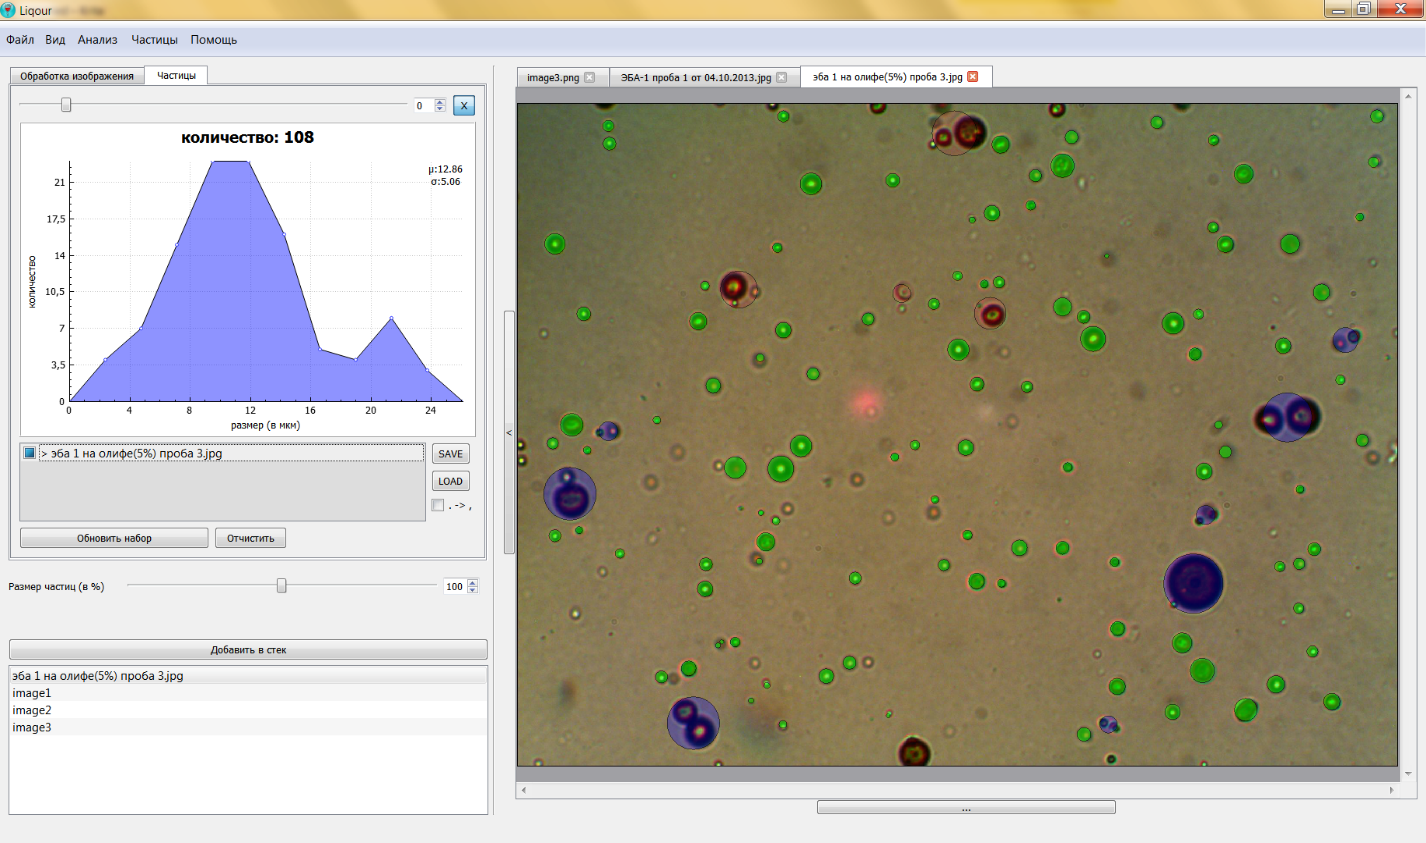
\includegraphics[scale=0.75]{images/em_05}
	\caption{ЭБА-1 на битуме разжиженном олифой (5\%)}
	\label{em_img_01}
\end{figure}

\begin{table}[h]
  \centering
  \caption{Распределение частиц на рис.\ref{em_img_01}}
  \renewcommand{\arraystretch}{1.5}% Spread rows out...Рис.9 Эмульсия, полученная в заводских условиях на вязком битуме.
  \begin{tabular}{*2{>{\centering\bfseries}m{1in}}>{\centering\arraybackslash}m{0.6in}}
    \toprule
	\textbf{Среднее значение, мкм.} & \textbf{Ср.кв. отклонение, мкм.} & \textbf{Всего частиц} \\
	\midrule
		\midrule
	12.86 & 5.06 & 108 \\
	\bottomrule
  \end{tabular}
\end{table}

Стандартные диспергаторы на которых дорожники производят битумные эмульсии позволяют получать средний размер частиц примерно 10 -20 мкм. Одним из возможных способов уменьшения размеров частиц эмульсии может являться понижение вязкости битума.
%
%\begin{figure}[h]
%	\centering
%	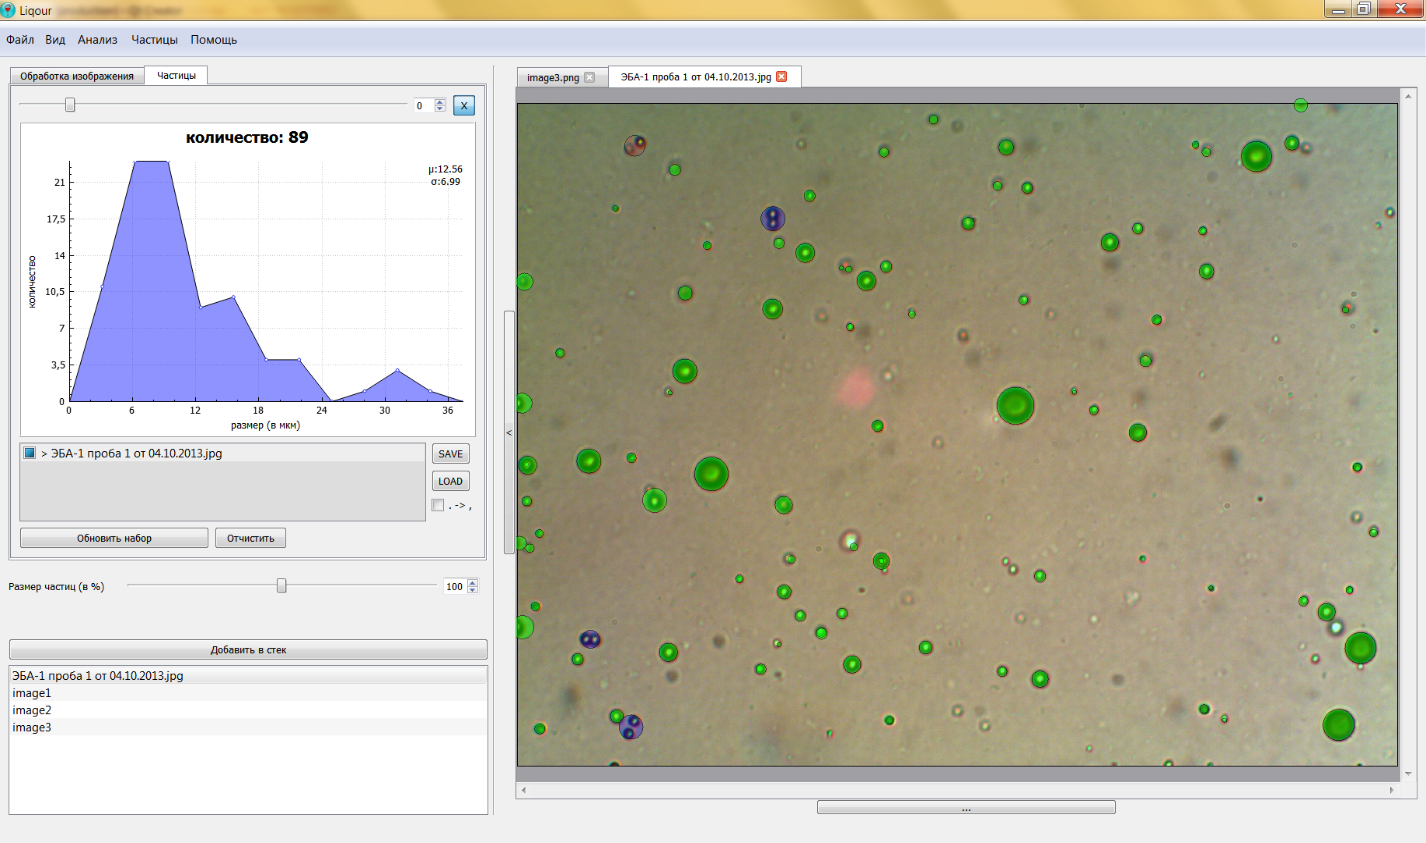
\includegraphics[scale=0.75]{images/em_06}
%	\caption{Эмульсия, полученная в заводских условиях на вязком битуме}
%	\label{em_img_02}
%\end{figure}
%
%\begin{table}[h]
%  \centering
%  \caption{Распределение частиц на рис.\ref{em_img_02}}
%  \renewcommand{\arraystretch}{1.5}% Spread rows out...Рис.9 Эмульсия, полученная в заводских условиях на вязком битуме.
%  \begin{tabular}{*2{>{\centering\bfseries}m{1in}}>{\centering\arraybackslash}m{0.6in}}
%    \toprule
%	\textbf{Среднее значение, мкм.} & \textbf{Ср.кв. отклонение, мкм.} & \textbf{Всего частиц} \\
%	\midrule
%	12.56 & 6.99 & 89 \\
%	\bottomrule
%  \end{tabular}
%\end{table}

\subsection{Результаты}
Разработанный программный комплекс, показал что изложенные выше алгоритмы отлично справляются с задачей классификации объектов по контору.

\section{Автоматизация составления ПОДД}
Работая с базой данных (БД) автомобильных дорог (далее а/д), было замечено, что большинство свойств а/д, можно отразить следующей схемой (рис. \ref{auto_scheme}, серая область). 

\begin{figure}[h]
	\centering
	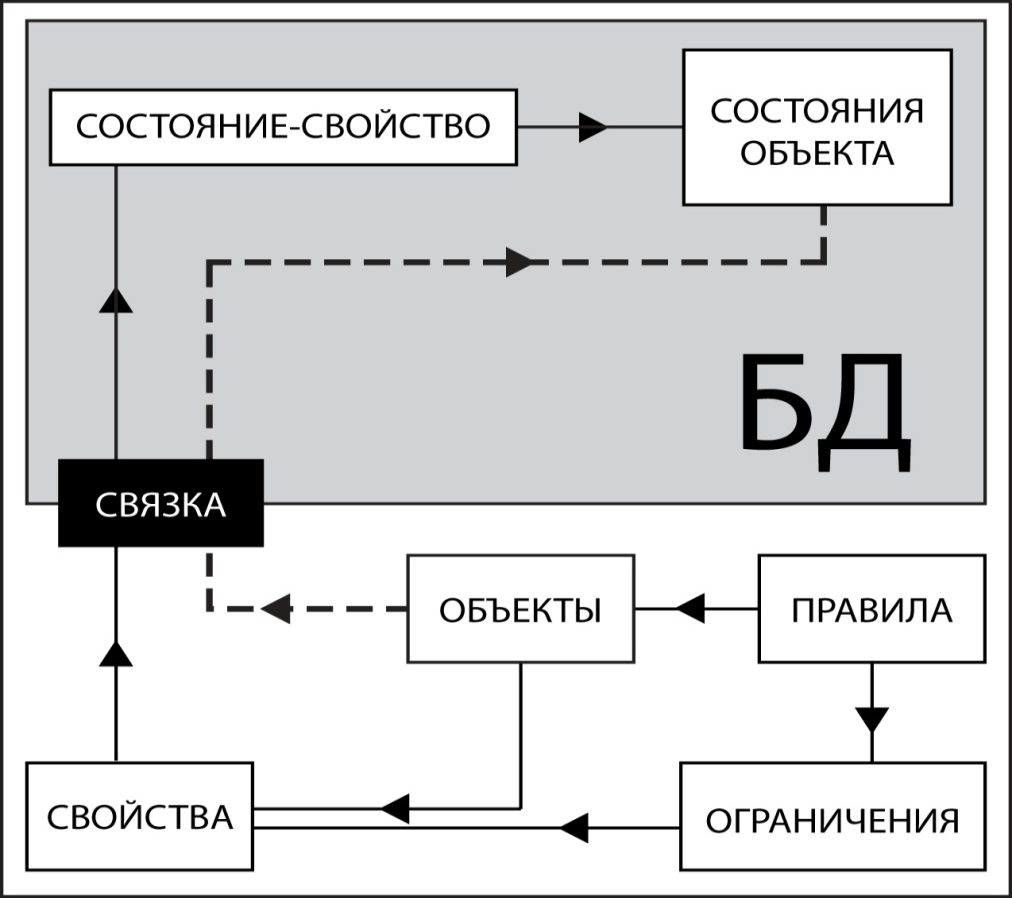
\includegraphics[scale=0.75]{images/auto_scheme}
	\caption{Схема представления свойств автомобильной дороги}
	\label{auto_scheme}
\end{figure}
\noindent
где состояние – это некоторый участок АД, а свойство - это функция, протяженная на этом участке и соответствующая некоторому свойству дороги (причем в качестве свойств может выступать наличие на участке трубы, дорожного знака, съезда и т.д.). Стоит отметить, что в БД функция представлена, как правило, набором аппроксимирующих точек.

В соответствии с таким подходом, было решено разработать надстройку над БД, представляющую собой набор фиксированных таблиц, и осуществляющую связь с основной БД, через таблицу «связка». Таблица «связка» имеет ключевое значение в схеме. За счет неё организуется «безболезненная» связь между основной БД и надстройкой.

\begin{table}[h]
  \centering
  \caption{Таблица связки}
  \renewcommand{\arraystretch}{1.5}
  \begin{tabular}{*2{>{\centering\bfseries}m{1.5in}}>{\centering\arraybackslash}m{2in}}
    \toprule
	\textbf{id} & \textbf{имя таблицы в связи} & \textbf{имя поля содержащего значение в таблице связи} \\
	\midrule 
	\midrule
	\#\# & состояние-свойство & значение \\
	\bottomrule
  \end{tabular}
\end{table}

\begin{table}[t]
  \centering
  \caption{Таблица правил}
  \renewcommand{\arraystretch}{1.5}
  \begin{tabular}{*3{>{\centering\bfseries}m{1in}}>{\centering\arraybackslash}m{2in}}
    \toprule
	\textbf{id правила} & \textbf{id объекта} & \textbf{наименование}  & \textbf{id списка ограничений} \\
	\midrule 
	\midrule
	\#\# & \#\# & ГОСТ \#\#\#\#   & \#\#  \\
	\bottomrule
  \end{tabular}
\end{table}

\begin{table}[b]
  \centering
  \caption{Таблица ограничений}
  \renewcommand{\arraystretch}{1.5}
  \begin{tabular}{*2{>{\centering\bfseries}m{1in}}>{\centering\arraybackslash}m{2in}}
    \toprule
	\textbf{id ограничения} & \textbf{id свойства} & \textbf{значение} \\
	\midrule 
	\midrule
	\#\# & \#\# & асфальт  \\
	\bottomrule
  \end{tabular}
\end{table}

Так как схема разрабатывалась для общего случая автоматизация размещения подобъектов (т.е. в нашем случае дорожных ограждений, сигнальных устройств и т.д.) на протяженном объекте (а/д), то стоить разъяснить значения некоторые таблицы. 

Таблица «объекты» хранит все возможные протяженные объекты, на которых будут размещаться подобъекты. В нашем случае, в таблице будет только одна строка, соответствующая АД. Таблица «состояния объекта» хранит всевозможные участки АД (т.е. например Иркутск-Листвянка, Братск-Усть-Илимск и т.д.). 

Таблица «состояние-свойство» хранит множество функций-свойств (высота насыпи, тип покрытия и т.д.) для каждого конкретного глобального участка (состояния) АД. Об особенностях представления правил будет сказано ниже.
\subsection{Представление дороги}
Для представления а/д, заданной на промежутке,  используется система функций:
$$
Road = \begin{cases}
g_1(x), x \in [a, b] \\
g_2(x), x \in [a, b] \\
\dots \\
g_n(x), x \in [a, b]
\end{cases}
$$
где $g_i(x)$ соответствует $i$-му свойству. Если свойство есть некоторая постоянно изменяющиеся величина (например «высота насыпи»), то функция имеет вид непрерывной кривой и при технической реализации представляет собой набор аппроксимирующих точек. Если же свойство представляет собой величину, которая может принимать значения только из строго заданного набора (например «тип покрытия»), то функция имеет ступенчатый вид. 

\begin{figure}[h]
	\centering
	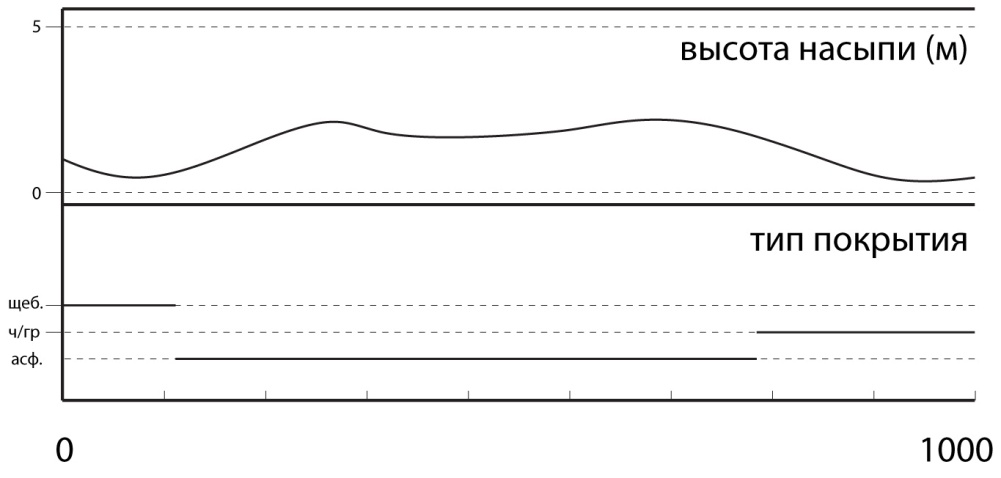
\includegraphics[scale=0.75]{images/auto_prop_graph.jpg}
	\caption{графики свойств}
	\label{auto_prop_graph}
\end{figure}
\subsection{Представление правил}
В отличие от данных а/д, информацию о правилах в БД хранить не принято. Связанно это с тем что, при составлении ПОДД, вся ответственность о корректности расположения тех или иных объектов на дороге ложится на плечи проектировщика, который прекрасно владеет правилами, и в случае необходимости обращается к ГОСТам. С другой стороны, чтобы научить машину расставлять объекты на плане в соответствии с ГОСТами в автоматическом режиме, мы должны эти ГОСТы положить в БД. 

Тут мы сталкиваемся с первой проблемой: с формальным представлением правила (т.е. как нам представить правило, чтобы его можно было хранить в БД). Так как каждое правило это есть некоторый набор конкретных значений свойств АД, то мы и будем представлять правило просто как набор значений:

$$
P_j = (p_{j_1}, \dots, p_{j_n})
$$

где каждая $p_{j_i}$ есть константа и соответствует $i$-му свойству $j$-го правила. В более сложных случаях, например, когда значение свойства может принимать значения из некоторого заданного промежутка, можно заменить константы векторами:

$$
P_j = (\overline{p_{j_1}}, \dots, \overline{p_{j_n}})
$$

где $\overline{p_{j_i}} = (a_{j_i}, b_{j_i})$ и соответствует $i$-му свойству $j$-го правила. Оба варианта легко реализуются в рамках СУБД. 


Вторая проблема заключается в том, как ГОСТ привести к формальному виду. Рассмотрим решение данной проблемы на примере ГОСТ 52289 пункта 8, правила применения дорожных ограждений и направляющих устройств. Так как постановка задачи требует от нас найти корректное расположение для некоторого объекта на АД, то можно пренебречь некоторыми правилами  определяющими качественное представление объекта (напр.: кол-во направляющих устройств, удерживающая способность и т.д.). 

В качестве наглядного представления формализованного правила удобно использовать блок-схемы. 

\begin{figure}[h]
	\centering
	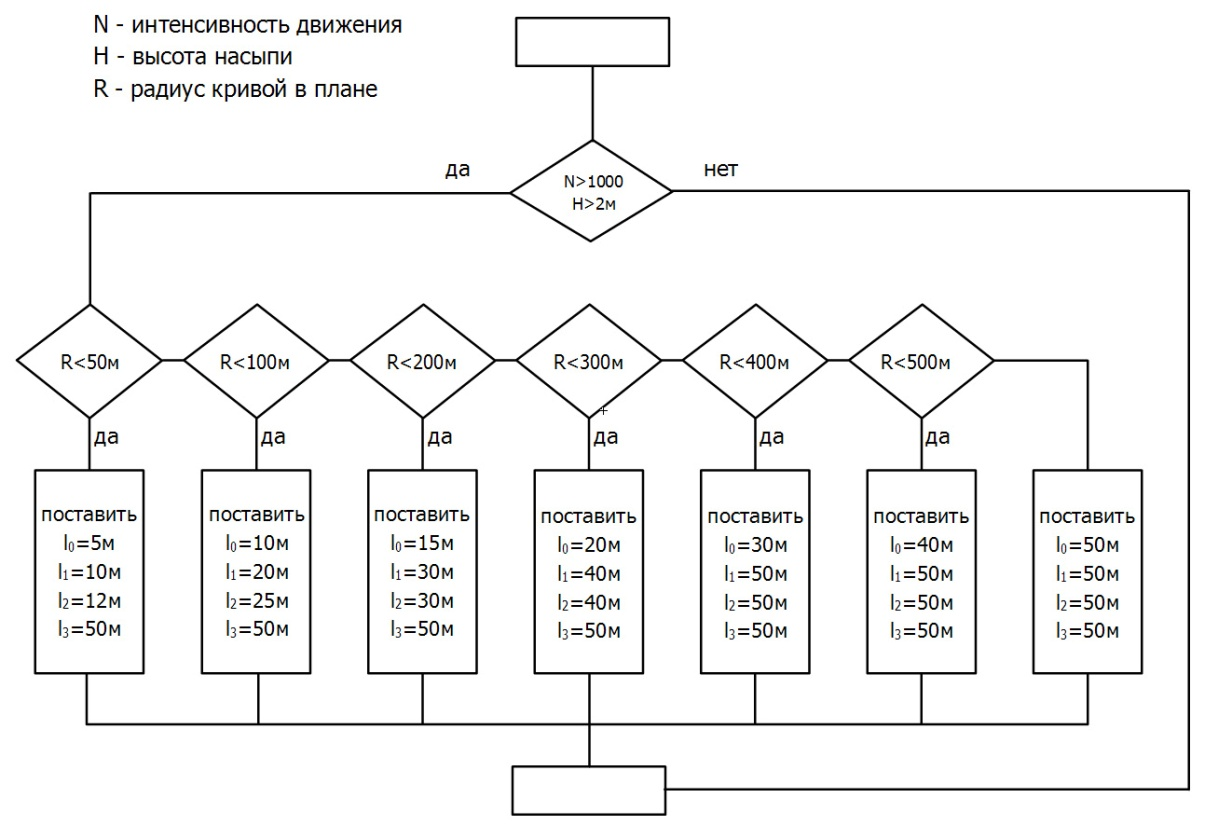
\includegraphics[scale=1]{images/auto_scheme_2}
	\caption{Блок схема определяющая ГОСТ 52289 пункта 8}
	\label{auto_scheme_2}
\end{figure}

На рис. \ref{auto_scheme_2}. приведена часть схемы для расстановки сигнальных устройств на АД. Каждый возможный «путь» в этой схеме будет соответствовать одной строке в таблице правил БД. 

\subsection{Автоматизация}
Разработанная система представления, позволяет нам реализовать схему автоматизированного расставления объектов на плане АД. Для начала рассмотрим простой пример, который позволит нам лучше разъяснить принцип работы. Пусть АД определена в базе двумя функциями-свойствами $A$ и $B$ и задано два правила:
$$
P_1 = [(a_1, a_2), b_1]
$$
$$
P_2 = [(a_2, a_3), b_2]
$$
\begin{figure}[h]
	\centering
	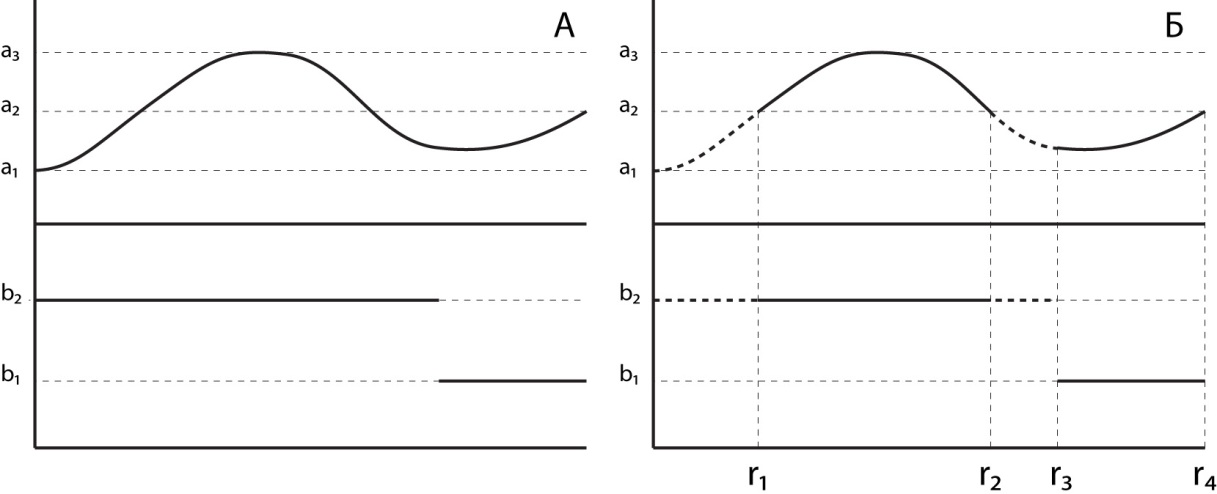
\includegraphics[scale=1]{images/auto_grap3}
	\caption{Объединеные графики свойств}
	\label{auto_graph3}
\end{figure}

На рис. \ref{auto_graph3} А представлены графики функций-свойств $A$ (верхний) и $B$ (нижний) на некотором участке дороги. Наша задача найти промежутки удовлетворяющие заданным выше правилам. Мы разбиваем участок на под-участки точками пересечения функций $A(x)$ и $B(x)$ с прямыми $y = a_1$, $y = a_2$, $y = a_3$ и $y = b_1$, $y = b_2$ соответственно. 

В результате обнаруживаем (рис. \ref{auto_graph3} Б), что промежуток $[r_1,r_2]$ удовлетворяет правилу $P_2$, а промежуток $[r_3,r_4]$ удовлетворяет правилу $P_1$. После того как промежутки найдены, остается подобрать объекты для которых выполнения любого из правил $P_1$ и $P_2$ достаточно для того, чтобы их расположение соответствовало правилам ГОСТ, и поставить их на плане АД. 

Формально автоматизацию можно описать следующим образом. Дорога представлена системой функций
$$
Obj = 
\begin{cases}
g_1(x), x \in [a, b] \\
g_2(x), x \in [a, b] \\
\dots \\
g_n(x), x \in [a, b]
\end{cases}
$$
\noindent
заданной в двумерном пространстве на промежутке $[a,b]$. Функции $g_i(x)$ будем называть свойствами объекта. Функции $g_1(x)$ являются непрерывными по $X$ на промежутке $[a,b]$. Требуется найти промежутки из $[a,b]$, на которых объект удовлетворяет ограничениям. Пусть $A_i$ как области значений функций определяющих ограничение:
$$
A_i = E(f_i(x)), i = \overline{1, n}
$$
где $f_i(x)$ -- функции заданные на некотором промежутке  Ограничения будем представлять следующим образом:

$$
\begin{aligned}
	R_j = \begin{cases}
	f_1(x_j) \\
	f_2(x_j) \\
	\dots \\
	f_n(x_j)
	\end{cases},\;
\end{aligned}
\begin{aligned}
j = \overline{1, m}
\end{aligned}
$$

\textbf{Этап 1.} Сведение объекта  к новому объекту заданному ступенчатыми функциями.
$$
\begin{aligned}
	Obj_2 = 
	\begin{cases}
		h_1(x), x \in [a, b] \\
		h_2(x), x \in [a, b] \\
		\dots \\
		h_n(x), x \in [a, b]
	\end{cases}
\end{aligned}
\begin{aligned}
h_i = \{x\;|\; f_i(x_{j_1}) \leq g_i(x) < f_i(x_{j_2}) \}
\end{aligned}
$$

Оценка: сложность осуществления перехода порядка $O(m)$.


\textbf{Этап 2.} Разбиение объекта  на множество подобъектов $\{obj_k\}$.
Данный шаг позволяет нам перейти от объекта заданного системой функций к множеству подобъектов, каждый из которых определен системой констант. Такое разбиение позволяет нам реализовать методы проверки ограничений, который подробно были рассмотрены в предыдущих работах [3]. 

Пусть $s_i$ -- кол-во точек разрыва у функции $h_i(x)$ на $[a, b]$. $S = \sum_{i}s_i$ -- это общее кол-во точек разрыва на $[a,b]$ у всех функций $h_i(x)$ вместе взятых. 

Пусть $\{x_1, \dots, x_S\}$ -- упорядоченное по возрастанию множество точек разрыва. Тогда наше множество подобъектов будет задано следующим образом:
 
$$
\begin{aligned}
	obj_i = 
	\begin{cases}
		h^+_1(x_i), x \in [x_i, x_{i+1}] \\
		h^+_2(x_i), x \in [x_i, x_{i+1}] \\
		\dots \\
		h^+_n(x_i), x \in [x_i, x_{i+1}]
	\end{cases}
\end{aligned}
\begin{aligned}
\text{при } i < S - 1
\end{aligned}
$$
и
$$
\begin{aligned}
	obj_i = 
	\begin{cases}
		h^+_1(x_i), x \in [x_i, b] \\
		h^+_2(x_i), x \in [x_i, b] \\
		\dots \\
		h^+_n(x_i), x \in [x_i, b]
	\end{cases}
\end{aligned}
\begin{aligned}
\text{при } i = S - 1
\end{aligned}
$$
Отметим что $x_1 = a, x_s = b$. Сложность построения нового множества объектов порядка $O(S)$.

Оценки позволяют сделать вывод о возможности эффективной реализации предложенного метода.
Результаты
Система автоматизации проектирования ПОДД успешно использовалась при выполнении контрактов составления  ПОДД для а/д  «Иркутск-Листвянка», «Братск-Усть-Илимск» и других. 

%
%\section{Таблица обыкновенная} \label{sect3_1}
%
%Так размещается таблица:
%
%\begin{table} [htbp]
%  \centering
%  \parbox{15cm}{\caption{Название таблицы}\label{Ts0Sib}}
%%  \begin{center}
%  \begin{tabular}{| p{3cm} || p{3cm} | p{3cm} | p{4cm}l |}
%  \hline
%  \hline
%  Месяц   & \centering $T_{min}$, К & \centering $T_{max}$, К &\centering  $(T_{max} - T_{min})$, К & \\
%  \hline
%  Декабрь &\centering  253.575   &\centering  257.778    &\centering      4.203  &   \\
%  Январь  &\centering  262.431   &\centering  263.214    &\centering      0.783  &   \\
%  Февраль &\centering  261.184   &\centering  260.381    &\centering     $-$0.803  &   \\
%  \hline
%  \hline
%  \end{tabular}
%%  \end{center}
%\end{table}
%
%%\newpage
%%============================================================================================================================
%
%\section{Параграф - два} \label{sect3_2}
%
%Некоторый текст.
%
%%\newpage
%%============================================================================================================================
%
%\section{Параграф с подпараграфами} \label{sect3_3}
%
%\subsection{Подпараграф - один} \label{subsect3_3_1}
%
%Некоторый текст.
%
%\subsection{Подпараграф - два} \label{subsect3_3_2}
%
%Некоторый текст.
%
%\clearpage